





% 下面方法是 vlm-based 的人形vla的文章
% https://arxiv.org/pdf/2603.12263
% https://arxiv.org/pdf/2607.18016
% https://arxiv.org/pdf/2503.14734
% https://arxiv.org/pdf/2608.16837
% https://arxiv.org/pdf/2510.03022
% https://arxiv.org/pdf/2606.22174
% https://arxiv.org/pdf/2603.05410
% https://arxiv.org/pdf/2603.09170v1

% 下面方法是 vgm-based 的人形vla 的文章
% https://arxiv.org/pdf/2608.06375
% https://arxiv.org/pdf/2606.09215
% https://arxiv.org/pdf/2609.16644v1

% 逻辑
Vision--language--action (VLA) models integrate visual perception, language understanding, and action generation across manipulation tasks and robot embodiments~\cite{rt2,openvla,pi0,wang2026limitsvisionandlanguagenavigation,wang2025dreamnavtrajectorybasedimaginativeframework}.
Learning instruction-conditioned behaviors from demonstrations provides a unified mapping from multimodal inputs to robot actions.
Extending VLA learning to humanoids could broaden task coverage in human environments, where locomotion, posture, and manipulation must be coordinated~\cite{grootn1,psi0,openhlm}.
For example, transferring objects between tables requires grasping, turning, walking, and placement while maintaining balance (Fig.~\ref{fig:overview}, bottom).
Such tasks require grounding task intent and visual feedback in coherent whole-body actions, motivating the extension of robot policy architectures to humanoid loco-manipulation.





% 逻辑：
% 1. 从机械臂操作走向人形全身控制
% 2. 引入现有方法两种骨干选择 (图 2(a)(b))
% 3. 阐述现有的动作预测方式 (图 2(c)(d))
% 4. 阐述现有方法的优势
Humanoid policy learning commonly extends the backbone--action expert paradigm from manipulation to whole-body control.
Pretrained vision--language models encode instruction and observation semantics (Fig.~\ref{fig:policy_routes}(a))~\cite{grootn1,psi0,openhlm}, while video generators supply spatiotemporal priors for scene evolution (Fig.~\ref{fig:policy_routes}(b))~\cite{motionwam,wholebodywam_wbc}.
These representations condition action generation across root, body, and hand motion.
Unified predictors generate whole-body sequences (Fig.~\ref{fig:policy_routes}(d))~\cite{openhlm,motionwam}; hybrid designs combine upper-body joint targets with lower-body locomotion commands executed by dedicated controllers (Fig.~\ref{fig:policy_routes}(e))~\cite{humanoidexo,wholebodyvla}.
The former captures cross-component dependencies; the latter couples upper-body control with learned locomotion and stabilization.
Both transfer pretrained semantic and visual dynamics knowledge to humanoid loco-manipulation.


\suppressfloats[t]
\begin{figure*}[t]
  \centering
  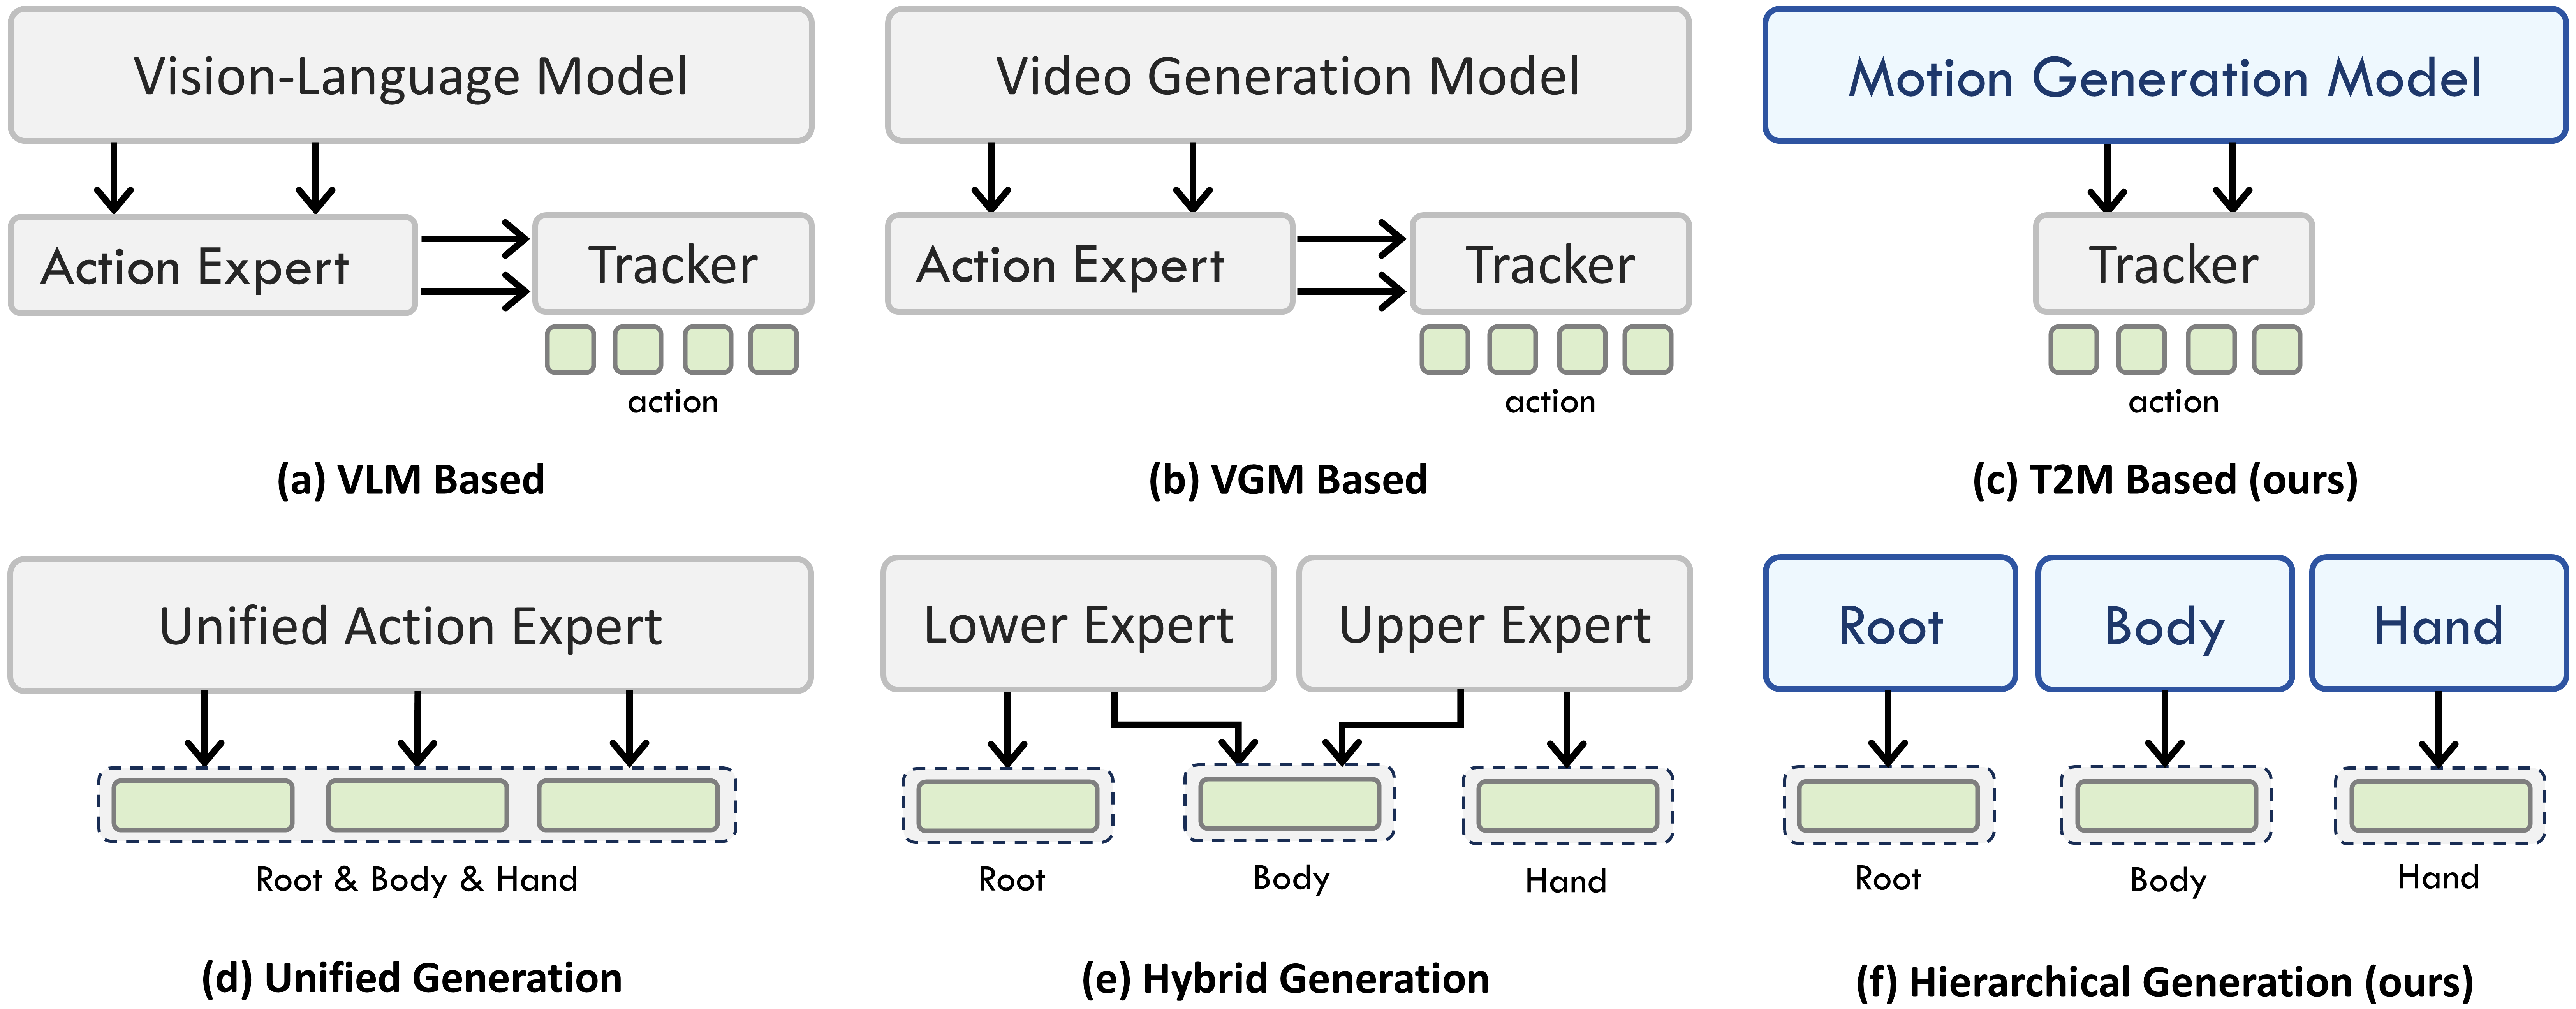
\includegraphics[width=0.98\textwidth]{image/intro_2.png}
  \caption{\textbf{Comparison of Humanoid Policy Architectures.}
  Panels (a)--(c) contrast VLM-based, VGM-based, and our T2M-based policy backbones.
  Panels (d)--(f) illustrate unified whole-body generation, hybrid generation of upper-body joint targets and lower-body locomotion commands, and our hierarchical root--body--hand generation, respectively.}
  \label{fig:policy_routes}
\end{figure*}



% 逻辑：
% 1. 承上起下：尽管上述方法能够迁移语义与视觉动态知识，但将其用于人形全身控制，仍面临运动先验与动作建模两方面的挑战
% 2. 阐述问题1：人形全身运动先验不足。 相较于固定基座机械臂操作，人形全身控制需要在同一动作序列中建模更高维、强耦合的运动关系。然而，VLM/VGM 预训练主要提供语义理解与视觉动态知识，并不直接赋予动作生成模块相应的全身运动先验。因此，迁移后的动作专家仍需从有限的人形示范中学习跨关节协调与时序结构，承担较大的学习负担。
% 3. 阐述问题2: 动作差异化建模不足。 根部移动、身体姿态与手部操作具有不同的运动尺度和精度要求，而统一预测与部分解耦架构仍由共享动作专家联合建模全部或部分运动分量，未充分体现这些差异。这种建模方式可能引入不同控制目标之间的学习干扰，增加兼顾局部动作精度与全身协调的难度。

% Despite these advances, transferring semantic and visual dynamics knowledge to humanoid whole-body control presents two challenges.
% \textbf{\ding{182} Insufficient Whole-Body Motion Priors.}
% Compared with fixed-base manipulation, humanoid control requires modeling higher-dimensional, strongly coupled motion across body parts and time within each action sequence.
% Existing systems initialize their representation backbones from vision--language, video-dynamics, or world--action pretraining~\cite{grootn1,psi0,motionwam,wholebodywam_wbc}.
% However, such backbone pretraining does not itself provide the action generator with a whole-body motion prior aligned with the target humanoid's kinematic space. When target-humanoid demonstrations are limited, the action expert must therefore acquire inter-joint coordination and temporal structure during policy adaptation.
% \textbf{\ding{183} Insufficient Differentiation of Motion Components.}
% Root motion, body articulation, and hand control operate at different motion scales and require different levels of precision.
% Unified action generators place these heterogeneous components within a shared prediction process~\cite{openhlm,motionwam}. Because root, body, and hand motions differ in scale and precision, this shared formulation may create competition between their learning objectives.
% Hybrid designs separate upper-body joint targets from lower-body locomotion commands~\cite{humanoidexo,wholebodyvla}. However, this execution-level split does not itself provide specialized generation pathways for root, body, and hand motion.
% These designs therefore leave substantial demands on the action predictor to accommodate component-specific requirements while learning the dependencies needed for whole-body coordination.

Despite these advances, two challenges remain.
\textbf{\ding{182} Insufficient Whole-Body Motion Priors.}
Compared with fixed-base manipulation, humanoid control requires higher-dimensional inter-joint and temporal coordination. Backbone pretraining~\cite{grootn1,psi0,motionwam,wholebodywam_wbc} does not directly equip action generators with priors aligned with target humanoid kinematics, leaving them to learn these priors, often from limited task-specific demonstrations.
\textbf{\ding{183} Insufficient Differentiation of Motion Components.}
Root, body, and hand control differ in scale and precision. Unified prediction~\cite{openhlm,motionwam} may create competing objectives; hybrid execution~\cite{humanoidexo,wholebodyvla} does not itself provide dedicated root, body, and hand generators. Both must accommodate component-specific requirements while maintaining whole-body coordination.


% 逻辑 
% 1. 提出并概述方法, 对应图 1 上部
% 2. 回应问题1，强动作先验: 选择 T2M 骨干，对应图 2(c)
% 3. 回应问题2, 强: 3阶段框架, 对应图 2(f)

Recent text-to-motion (T2M) methods learn structured motion distributions conditioned on text or spatial constraints~\cite{temos,mdm,mld,t2mgpt,momask,omnicontrol}.
Building on these advances, \textbf{Kimodo-Policy} combines a pretrained T2M backbone with three-stage root--body--hand generation for humanoid VLA control.
\textbf{\ding{182} Strong Whole-Body Motion Priors.}
We transfer Kimodo's pretrained inter-joint and temporal priors to high-dimensional, visually grounded control (Fig.~\ref{fig:policy_routes}(c))~\cite{kimodo}, easing motion learning from limited task-specific humanoid demonstrations.
\textbf{\ding{183} Strong Component-Specific Motion Modeling.}
Dedicated generators (Fig.~\ref{fig:policy_routes}(f)) predict root translation and heading, root-conditioned body motion, and hand controls conditioned on future body features and visual observations. Their dependencies support component specialization and whole-body coordination.
We pretrain on diverse humanoid demonstrations to generate actions conditioned on visual observations, language instructions, and motion history.
With 678M total and only 92M trainable parameters, Kimodo-Policy shows consistent gains from more VLA pretraining data, larger models, and stronger T2M priors. Our main contributions are:
\begin{itemize}
  \item We introduce \textbf{Kimodo-Policy}, a humanoid VLA framework that transfers pretrained T2M motion priors to visually guided whole-body control. VLA pretraining on diverse humanoid demonstrations grounds these priors in visual observations, language instructions, and motion history for closed-loop execution.

  \item We propose a three-stage root--body--hand architecture with dedicated generators that accommodate distinct control requirements. Explicit cross-stage conditioning preserves dependencies among motion components, supporting specialized generation and whole-body coordination.
  
  \item We demonstrate strong performance on HumanoidArena, SIMPLE, and real-world humanoid tasks with 678M total and only 92M trainable parameters. Scaling studies show consistent gains from larger VLA pretraining datasets, greater model capacity, and stronger pretrained T2M priors.
\end{itemize}
